\documentclass[a4paper,12pt]{article}

\usepackage[left=2cm, right=2cm, top=3cm, bottom=3cm]{geometry} %Para poner los márgenes


\usepackage{float} %Para hacer que la megatabla no se vaya volando a la última página y forzar que se quede usando [H]

% Idioma español y codificación
\usepackage[spanish]{babel} % Traduce palabras como "Contenido", "Capítulo", etc.
\usepackage[utf8]{inputenc} % Permite escribir caracteres en español (á, é, ñ, etc.)
\usepackage[T1]{fontenc}    % Mejora la salida de caracteres acentuados en PDF

% Paquetes matemáticos
\usepackage{amsmath}  % Permite usar comandos avanzados de matemáticas
\usepackage{amssymb}  % Agrega símbolos matemáticos adicionales
\usepackage{amsthm}   % Permite definir teoremas, lemas, etc.
\usepackage{mathrsfs} % Fuente adicional para letras matemáticas

% Para mejor tipografía en matemáticas
\usepackage{mathtools}

% Si necesitas gráficos
\usepackage{graphicx} 

% Si usas referencias cruzadas en el documento
\usepackage[hidelinks]{hyperref}  % Enlaces clicables en PDF

%Para poner el color de los enlaces azul
\hypersetup{
    colorlinks=true,       % Habilita los enlaces de colores
    linkcolor=black,        % Color de los enlaces internos (por ejemplo, referencias a secciones)
    urlcolor=magenta,      % Color de los enlaces a direcciones web
    citecolor=red,         % Color de las referencias bibliográficas
    filecolor=cyan,        % Color de los enlaces a archivos
}

\renewcommand{\contentsname}{Índice} % Cambia "Contenido" por "Índice"

\usepackage{listings}
\usepackage{xcolor} % Para definir colores, opcional

% Configuración básica de listings:
\lstset{
    language=C,                    % Especifica el lenguaje (puede ser Python, Java, etc.)
    basicstyle=\ttfamily\small,     % Fuente de tipo monoespaciada
    numbers=left,                  % Números de línea a la izquierda
    numberstyle=\tiny,             % Estilo de los números de línea
    stepnumber=1,                  % Mostrar número en cada línea
    numbersep=10pt,                % Espacio entre número y código
    backgroundcolor=\color{lightgray}, % Color de fondo
    showspaces=false,              % No resaltar espacios
    showstringspaces=false,        % No resaltar espacios en cadenas
    showtabs=false,                % No resaltar tabulaciones
    frame=single,                  % Agregar un marco alrededor del código
    rulecolor=\color{black},       % Color del marco
    captionpos=b,                  % Posición de la leyenda (b de bottom)
    breaklines=true,               % Saltos automáticos de línea
    breakatwhitespace=false,
    title=\lstname,                % Muestra el nombre del archivo, si se especifica
    keywordstyle=\color{blue},     % Color de las palabras clave
    commentstyle=\color{purple},    % Color de los comentarios
    stringstyle=\color{red}        % Color de las cadenas
}

\usepackage{caption}
\captionsetup[table]{labelformat=empty} %Para que no salgan numeradas las tablas
\captionsetup[lstlisting]{labelformat=empty} %Para que no salgan numeradas los fragmentos de código
\captionsetup[table]{labelformat=empty} %Para que no salgan numeradas las tablas
\captionsetup[figure]{labelformat=empty} %Para que no salgan numeradas las gráficas
\setlength{\parindent}{0.75cm} %Para que la sangría no sea tan grande
 % Todos los preámbulos

% =====================
% Índice
% =====================
\begin{document}
\begin{titlepage}
	\centering

	
\includegraphics[width=0.3\textwidth]{Imagenes/logo_ugr.png} % Ajusta el tamaño según necesites (0.3\textwidth es solo un ejemplo)
	\vspace{1cm} % Ajusta el espacio según lo necesites

	{\bfseries\LARGE Universidad de Granada \par}
	\vspace{1cm}
	{\scshape\Large Facultad de Ingeniería Informática y telecomunicaciones \par}
	\vspace{3cm}
	{\scshape\Huge Práctica 1: Eficiencia de algoritmos \par}
	\vspace{3cm}
	{\itshape\Large Doble Grado Ingeniería Informática y Matemáticas \par}
	\vfill
	{\Large Autores: \par}
	{\Large Adolfo Martínez Olmedo, Pablo Delgado Galera, Marcos Baena Solar \par}
	\vfill
	{\Large Marzo 2025 \par}
\end{titlepage}
 % Archivo con la portada

\tableofcontents

\newpage

% =====================
\section{Introducción}
% =====================
En esta práctica se desarrolla la resolución de tres problemas diferentes: 

\begin{itemize}
	\item Menor número
	\item Menor distancia
	\item Menor envolvente convexa
\end{itemize}

Lo haremos de dos maneras distintas, primero haremos una aproximación mediante algoritmos 
de fuerza bruta y después aplicaremos lo aprendido en clase, desarrollando soluciones basadas 
en divide y vencerás. Analizaremos la eficiencia teórica de cada solución, mediante un script
ejecutaremos los programas con diferentes tamaños y una cantidad determinada de veces, nos 
quedaremos con una media de todas las ejecuciones y podremos comparar la eficiencia de ambas 
soluciones, viendo a partir de que tamaños es mejor una solución a la otra en cuanto a eficiencia.
\\

Para todas las ejecuciones de los diferentes algoritmos hemos usado el mismo portátil. Un \textit{Asus Zephyrus G14} con un procesador \textit{Ryzen 7 4800HS}, cuyas especificaciones se pueden ver en la siguiente imágen:\\
\begin{center}
	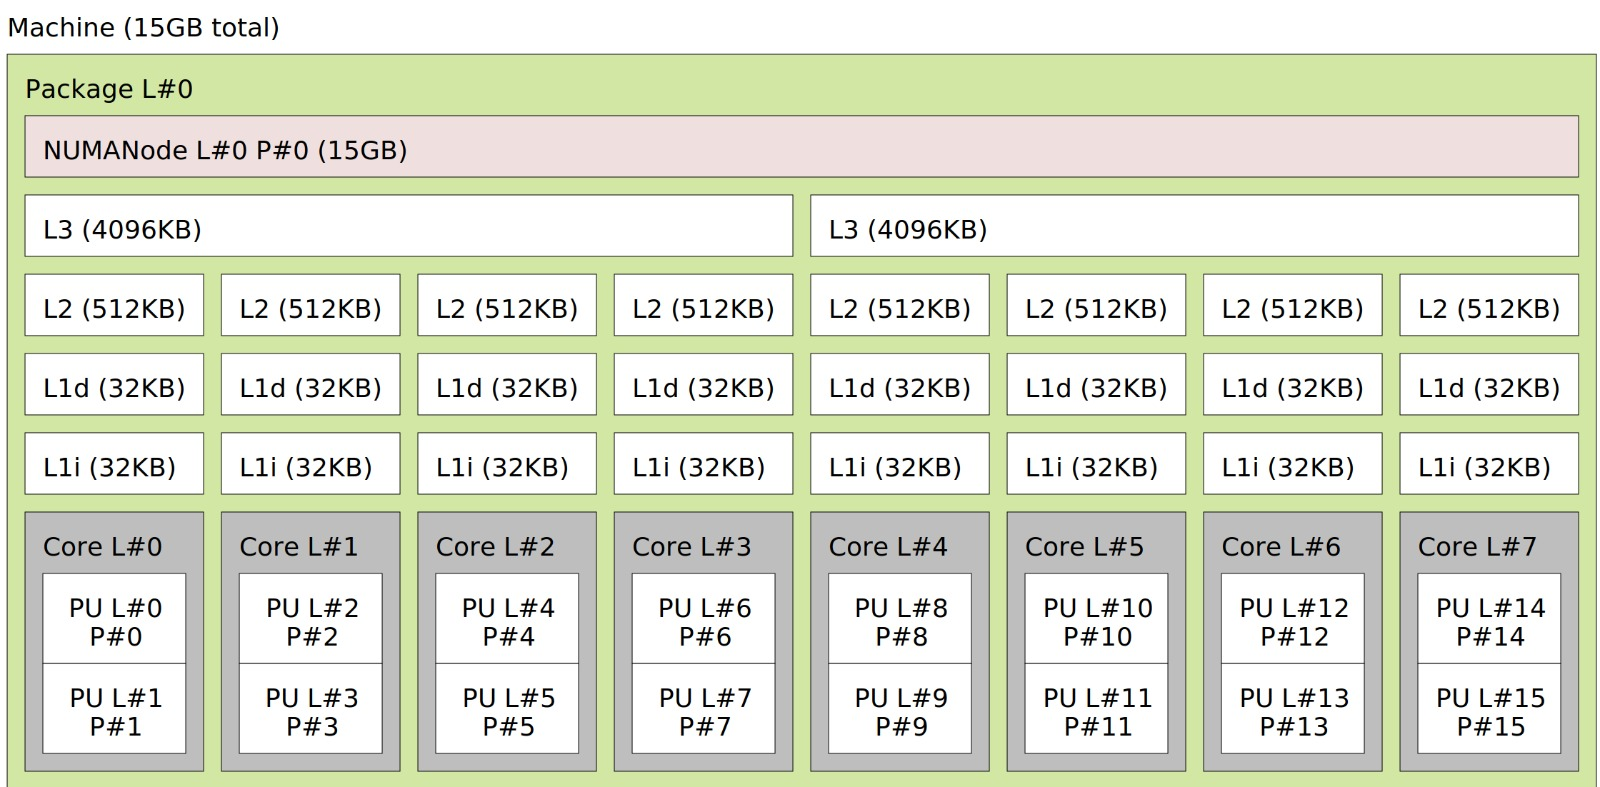
\includegraphics[width=0.8\textwidth]{Imagenes/lstopo.jpeg}
\end{center}



% =====================
\section{Objetivos}
% =====================
Los objetivos de esta práctica son los siguientes:
\begin{itemize}
	\item Comprender la técnica de Divide y Vencerás y sus ventajas.
	\item Comparar con la estrategia de fuerza bruta y analizar la complejidad.
	\item Implementar ambos enfoques (fuerza bruta y Divide y Vencerás) para cada problema.
	\item Experimentar con el umbral de la técnica de Divide y Vencerás.
\end{itemize}

% =====================
\section{El número más pequeño}
\label{sec:El número más pequeño}
% =====================
\subsection{Análisis de Fuerza Bruta}

Nuestra idea para desarrollar el algoritmo de fuerza bruta se basa en ir recorriendo el vector de 
puntos tantas veces como cifras tenga el número que busquemos, y en cada recorrido se busca el 
número más pequeño, se elimina y se procede a hacer lo mismo en la siguiente iteración, hasta obtener 
finalmente el número más pequeño posible, ejecutamos el programa con un valor de k entre 4 y 9, ya 
que el mayor entero que acepta C++ tiene 10 dígitos.\\

El código es el siguiente:

\begin{lstlisting}[language=C++, caption={Brute Force de \textbf{``El número más pequeño''}}]
int getSmallestNumber(std::vector<int> &v, int k) {
    
    int N = v.size();

    vector<int> copy(v);
    auto pos = copy.begin();
    string smallest_str = "";

    while (smallest_str.size() < k){
        int smallest = std::numeric_limits<int>::max();
        for (auto i = copy.begin(); i != copy.end(); ++i){ //encontramos minimo
            if (*i < smallest){
                smallest = *i;
                pos = i;
            }
        }
        smallest_str.append(to_string(smallest)); //append the min
        copy.erase(pos);
    }
    
    return (stoi(smallest_str));
}	
	 \end{lstlisting}

	 Tras el análisis teórico comprobamos que este código tiene una eficiencia de $O(k\cdot n)$, 
	 k al ser constante y menor que n no debería afectar a la eficiencia, tambén debido a la limitación 
	 impuesta por nosostros de que sea menor que 9, en un caso más general conforme crece la k se acercará a $O(n²)$.\\
	 
\subsection{Análisis de Divide y Vencerás}
Nuestra idea para desarrollar el algoritmo de Divide y Vencerás se basa en orderar el vector utilizando quickSort 
(para dividir y vencer) y una vez lo tenemos ordenado simplemente cogemos los k primeros números. \\

El código es el siguiente:

\begin{lstlisting}[language=C++, caption={Divide y vencerás de \textbf{``El número más pequeño''}}]
int getSmallestNumber(vector<int> v, int k)
{
	quicksort(v, 0, v.size() - 1);
	string result = "";
	for (int i = 0; i < k; ++i)
	{
		result += to_string(v[i]);
	}
	return stoi(result);
}	
	 \end{lstlisting}

Tras el análisis teórico comprobamos que este código tiene una eficiencia de $O(n\cdot \log (n))$, 
que ya conociamos de la práctica anterior, aunque debido a la cantidad de dígitos repetidos su eficiencia decae hasta casi $O(n²)$.\\

\subsection{Tablas y Gráficos de Rendimiento}

\begin{center}
	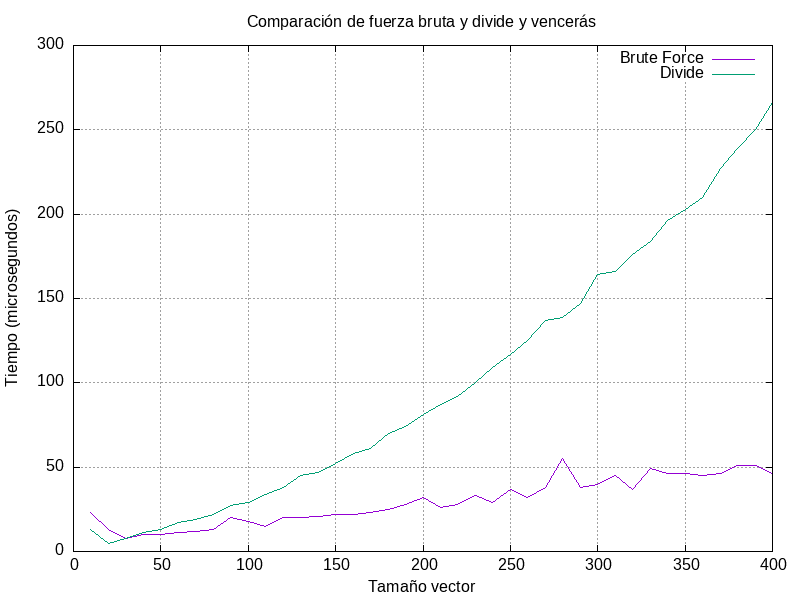
\includegraphics[width=0.8\textwidth]{scripts/smallest_number/Graficas/comparison_smallest_number.png}	
\end{center}


\subsection{Análisis de los Resultados}
Tras el analisis teórico y visualizar la gráfica comparativa, vemos que el algoritmo de Fuerza 
Bruta consigue resolver el problema de forma más eficiente que el algoritmo Divide y Vencerás. 
Esto se debe a que el primer algortimo depende de una constante k que consideramos siempre menor 
que n, y por tanto no afecta a la eficiencia. Mientras que en el segundo algoritmo podemos apreciar 
que quicksort tiene la eficiencia del peor caso, ya que al solo usar dígitos del 1 al 9, encontramos
en el vector una gran cantidad de números repetidos lo cual afecta gravemente a la eficiencia de este 
algortimo de ordenación.


% =====================
\section{El par de puntos más cercano}
% =====================
\subsection{Análisis de Fuerza Bruta}
Nuestra idea para desarrollar el algoritmo de fuerza bruta se basa en un doble bucle for el cual calcula todas 
las distancias de todos los puntos con todos, haciendo comparaciones hasta encontrar la mínima distancia. \\

El código es el siguiente:

\begin{lstlisting}[language=C++, caption={Brute Force de \textbf{``El par de puntos más cercan''}}]
double bruteForce(const vector<Point>& P, int l, int r) {
	double minDist = DBL_MAX;
	for (int i = l; i <= r; i++) {
		for (int j = i+1; j <= r; j++) {
			double d = dist(P[i], P[j]);
			if (d < minDist) {
				minDist = d;
			}
		}
	}
	return minDist;
}
\end{lstlisting}

Tras el análisis teórico comprobamos que este código tiene una eficiencia de $O(n^2)$.

\subsection{Análisis de Divide y Vencerás}
Nuestra idea para desarrollar el algoritmo de Divide y Vencerás se basa en ir haciendo divisiones
de un array de puntos previamente ordenado por la coordenada x de los puntos (de derecha a izquierda).
Tras esto, vamos haciendo divisiones partiendo el vector por la mitad recursivamente hasta quedarnos con 3 
puntos o menos en una franja, donde se resolverá el problema usando fuerza bruta. Así obtenemos la mínima distancia 
en una franja, tras esto nos quedamos con la mínima distancia entre la franja de la izquierda y la derecha, y la 
usaremos para estudiar la mínima distancia entre una franja intermedia de tamaño la mínima distancia, creamos esta franja 
con los puntos que estan a una distancia menor de la menor distancia previamente calculada respecto del punto central.
Una vez construido el strip comparamos los puntos con respecto a su coordenada y (esta comparación se hace con un 
número comnstante de puntos al reducirlos con la distancia mínima), se hace para evitar que puntos cercanos respecto a 
la coordenada x pero alejados respecto de la y sean los únicos que se comparan, buscando que sea menor que la menor distancia previa,
obtenemos así la mínima distancia entre la franja izquierda, derecha y central. Resolviendo recursivamente obtenemos 
la mínima distancia en un conjunto de puntos. \\

El código es el siguiente:

\begin{lstlisting}[language=C++, caption={Divide y vencerás de \textbf{``El par de puntos más cercano''}}]
double closestUtil(vector<Point> &PX, int l, int r) {
	// Si el subrango es peque, fuerza bruta
	if (r - l <= 3) {
		return bruteForce(PX, l, r);
	}

	int mid = (l + r) / 2;
	double midX = PX[mid].x;

	// bestPair se va actualizando; 
	// para tener la minima distancia, llamo recursivamente a izq y der
	double dl = closestUtil(PX, l, mid);
	double dr = closestUtil(PX, mid+1, r);

	double d = dl < dr ? dl : dr;
	// Construir el strip (puntos que quedan en [midX - d, midX + d])
	vector<Point> strip;
	strip.reserve(r - l + 1);
	for (int i = l; i <= r; i++) {
		if (fabs(PX[i].x - midX) < d) {
			strip.push_back(PX[i]);
		}
	}
	// Ordenar la franja por Y
	sort(strip.begin(), strip.end(), [](auto &a, auto &b){
		return a.y < b.y;
	});

	// Revisar cada punto del strip con sus siguientes
	// mientras la diferencia en Y sea < d
	for (int i = 0; i < (int)strip.size(); i++) {
		for (int j = i+1; j < (int)strip.size() && (strip[j].y - strip[i].y) < d; j++) {
			double distStrip = dist(strip[i], strip[j]);
			if (distStrip < d) {
				d = distStrip;
			}
		}
	}

	return d;
}
\end{lstlisting}

Para el análisis teórico de este algoritmo debemos estudiar la ecuación de recurrencia: $T(n) = 2T(\frac{n}{2}) + O(n)$.
Esta ecuación se obtiene de que una llamada a la función de tamaño n hará dos llamadas recursivas con cada mitad de los puntos (izquierda y derecha),
O(n) se obtiene de calcular los puntos en el strip central, que auqnue pueda parecer $O(n²)$, cada punto del strip solo 
se compara con un número constante de puntos, al habernos quedado previamente con una cantidad de puntos pequeñas dentro de un rango.
Cuando el tamaño es menor o igual que 3 (caso base), donde aplicamos 
fuerza bruta, al ser un tamaño tan pequeño, no afectará a la eficiencia.\\


Tras resolver la recurrencia comprobamos que este código tiene una eficiencia de $O(n\cdot \log (n))$.\\

\subsection{Tablas y Gráficos de Rendimiento}

\begin{center}
	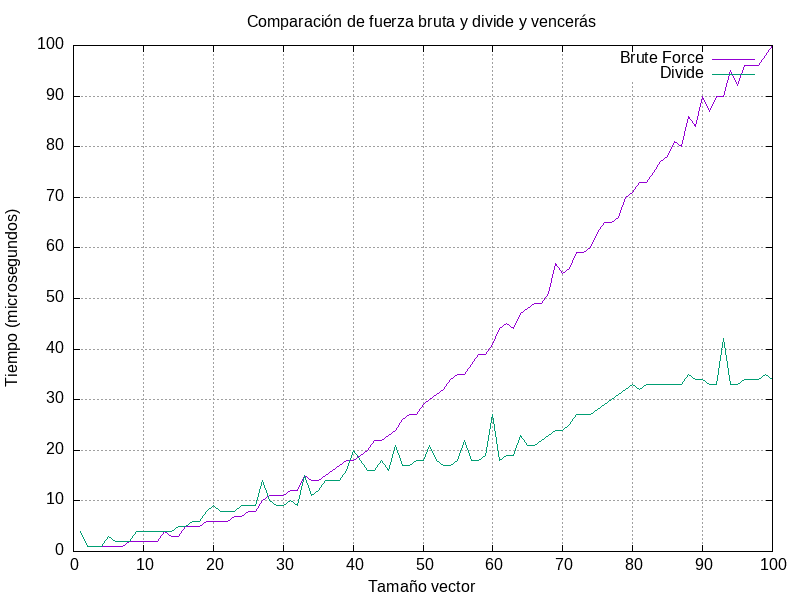
\includegraphics[width=0.8\textwidth]{scripts/closest_distance/Graficas/comparison_closest_distance.png}
\end{center}


\subsection{Análisis de los Resultados}
Como se esperaba tras el análisis teórico, en las gráficas podemos observar que el algoritmo Divide y Vencerás 
tiene una mayor eficiencia que el de Fuerza Bruta, también podemos observar la clara forma parábolica del algoritmo
Fuerza Bruta como habiamos previsto. También se puede observar la región a partir del cual el primer algortimo, comienza 
a tener tiempos de ejecución más bajos que el segundo.


% =====================
\section{La envolvente convexa}
% =====================
\subsection{Análisis de Fuerza Bruta}

Nuestra idea para desarrollar el algoritmo de fuerza bruta se basa en empezar seleccionando el punto más a la izquierda, 
el cual sabemos que siempre va a estar en la envolvente convexa, seguidamente seleccionas otro punto y compruebas si 
la recta que une los dos puntos deja el resto de puntos a la izquierda, una vez encuentras ese punto, es nuevo punto 
actúa como el primero que seleccionaste, y haces esto hasta que encuentres todos los puntos pertenecientes a la envolvente convexa. \\

El código es el siguiente:

\begin{lstlisting}[language=C++, caption={Brute Force de \textbf{``La envolvente convexa''}}]
// Estructura para representar un punto
struct Point {
float x, y;
};

typedef pair<int, int> ParPuntos;

// Funcion que calcula el convex hull por fuerza bruta
set<ParPuntos> convexHullBruteForce(const vector<Point>& points) {
int n = points.size();
set<ParPuntos> hull;

// Recorremos cada par de puntos
for (int i = 0; i < n; i++) {
	for (int j = i + 1; j < n; j++) {
	int left = 0, right = 0;
	
	// Verificamos la posicion de cada otro punto respecto a la linea formada por points[i] y points[j]
	for (int k = 0; k < n; k++) {
		if (k == i || k == j)
			continue;
			
		float position = (points[j].x - points[i].x) * (points[k].y - points[i].y) -
		(points[j].y - points[i].y) * (points[k].x - points[i].x);
		
		if (position > 0)
			left++;
		else if (position < 0)
			right++;
	}
	
	// Si todos los puntos se encuentran de un mismo lado (o son colineales), se adjuntan los puntos de la arista
	if (left == 0 || right == 0) {
		hull.insert({points[i].x, points[i].y});
		hull.insert({points[j].x, points[j].y});
	}
	}
}

return hull;
}
\end{lstlisting}

Tras el análisis teórico comprobamos que este código tiene una eficiencia de $O(n^3)$

\subsection{Análisis de Divide y Vencerás}
Nuestra idea para desarrollar el algoritmo de Divide y Vencerás se basa en ir diviendo los puntos del plano, previamente ordenados 
de derecha a izquierda, en dos partes (izquierda y derecha) hasta llegar a un tamaño pequeño donde se calculen las envolventes convexas,
tanto de izquierda como de derecha que se juntarán usando la función merge. Esta función comienza buscando de entre los puntos de la envolvente de la derecha 
el punto más a la izquierda, actuando analogamente con los de la izquierda, tras esto buscamos la tangente superior que cuyos puntos 
formarán parte de la envolvente. Para ello, vamos buscando con el punto más a la derecha de la izquierda fijo, y rotando el punto más a la 
izquierda de los derecha, ahcia la derecha hasta encontrar uno que deje el resto de puntos a la derecha, una vez lo encontramos fijamos 
ese punto y rotamos hacia la izquierda los puntos de la izquierda hasta encontrar uno que deje todos los puntos de la izquierda a la izquierda.
Repetimos para la tangente inferior rotando en sentido contrario, finalizamos guardando todoos los puntos resultantes en el vector a devolver. \\

El código es el siguiente:

\begin{lstlisting}[language=C++, caption={Divide y vencerás de \textbf{``La envolvente convexa''}}]
vector<Point> convexHullDC(vector<Point> &points, int l, int r) {
	// Base case: one point
	if (l == r) {
		return {points[l]};
	}
	// Base case: two points
	if (r - l == 1) {
		if (points[l].x == points[r].x && points[l].y == points[r].y)
			return {points[l]};
		return {points[l], points[r]};
	}
	int mid = (l + r) / 2;
	vector<Point> leftHull = convexHullDC(points, l, mid);
	vector<Point> rightHull = convexHullDC(points, mid + 1, r);
	return mergeHulls(leftHull, rightHull);
}
	
\end{lstlisting}

Para el análisis teórico de este algoritmo debemos estudiar la ecuación de recurrencia: $T(n) = 2T(\frac{n}{2}) + O(n)$.
Esta ecuación se obtiene de que una llamada a la función de tamaño n hará dos llamadas recursivas con cada mitad de los puntos (izquierda y derecha),
O(n) se obtiene de la llamada a la función merger que junta las dos envolventes con una eficiencia de O(n), ya que
hay se recorren varios bucles de la mitad del tamaño en cada iteración ($\frac{n}{2}$) obviando la constante obtenemos O(n).
El caso base usa la fuerza bruta en un conjunto de 5 puntos, su eficiencia es presecindible.

Tras resolver la recurrencia comprobamos que este código tiene una eficiencia de $O(n\cdot \log (n))$.

\subsection{Tablas y Gráficos de Rendimiento}

\begin{center}
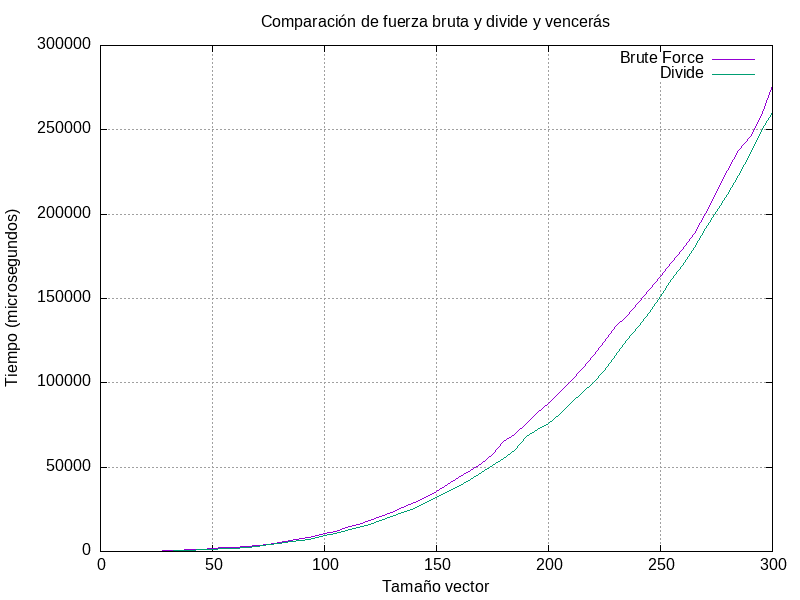
\includegraphics[width=0.8\textwidth]{scripts/convex_hull/Graficas/comparison_convex_hull.png}
\end{center}

\subsection{Análisis de los Resultados}
Como se esperaba tras el análisis teórico, en las gráficas podemos observar que el algoritmo Divide y Vencerás 
tiene una mayor eficiencia que el de Fuerza Bruta, también podemos observar la clara forma cúbica del algoritmo
Fuerza Bruta como habiamos previsto. También se puede observar la región a partir del cual el primer algortimo, comienza 
a tener tiempos de ejecución más bajos que el segundo.


En esta sección se describen los diferentes problemas que se abordarán.

% =====================
\section{Conclusiones}
% =====================
Tras esta práctica hemos descubierto que la estrategia de desarrollo de algoritmos Divide y Vencerás 
es útil en un amplio repertorio de casos pero esto no quiere decir que siempre sea mejor que un algoritmo 
fuerza bruta, esto lo podemos comprobar en \ref{sec:El número más pequeño}. Aún así en la gran mayoría de casos aplicar Divide y Vencerás 
supone una mejoría en la eficiencia del código.

\end{document}

